\documentclass[main.tex]{subfiles}
\begin{document}

\section{Umsetzung}
In diesem Abschnitt werden die Details der Implementationen auf den beiden Smartphone-Plattformen iOS und Android, sowie den Aufbau unserer ARDoor Library beschrieben.

\subsection{Grundarchitektur}
Wir haben die Grundarchitektur unserer Applikation laut der Abbildung \ref{fig:android-architecture} definiert. Die einzelnen Komponenten werden hier kurz beschrieben.

\paragraph{OpenCV}
ist ein quasi-Standard in der nativen Bildverarbeitung und unterstützt eine Vielzahl an Bearbeitungsfunktionen. OpenCV wird in der ARDoor Library für die Bildverarbeitung verwendet.

\paragraph{OpenGL}
wird für das 3D-Rendering benötigt. In der mobilen Welt ist die Library mittlerweile Standard und wird von Android und iOS unterstützt.

\paragraph{ARDoor C++ Library}
Die ARDoor Library enthält den Hauptteil der Applikation. In ihr wird sämtliche plattformunabhängige Logik sowie Verarbeitung und Rendering implementiert. C++ eignet sich  dafür gut, da sowohl von iOS via Objective-C als auch von Android über JNI auf die Library zugegriffen werden kann.

\paragraph{Plattformspezifischer Client}
Pro Plattform wird ein eigener Client implementiert, der den Kamerazugriff übernimmt. Die erfassten Einzelbilder werden an die ARDoor Library zur verarbeitung weitergereicht. Dieser Client sollte nur als Zwischenschicht dienen und deshalb so schlank wie möglich gehalten werden. 


\begin{figure}[!ht]
\centering
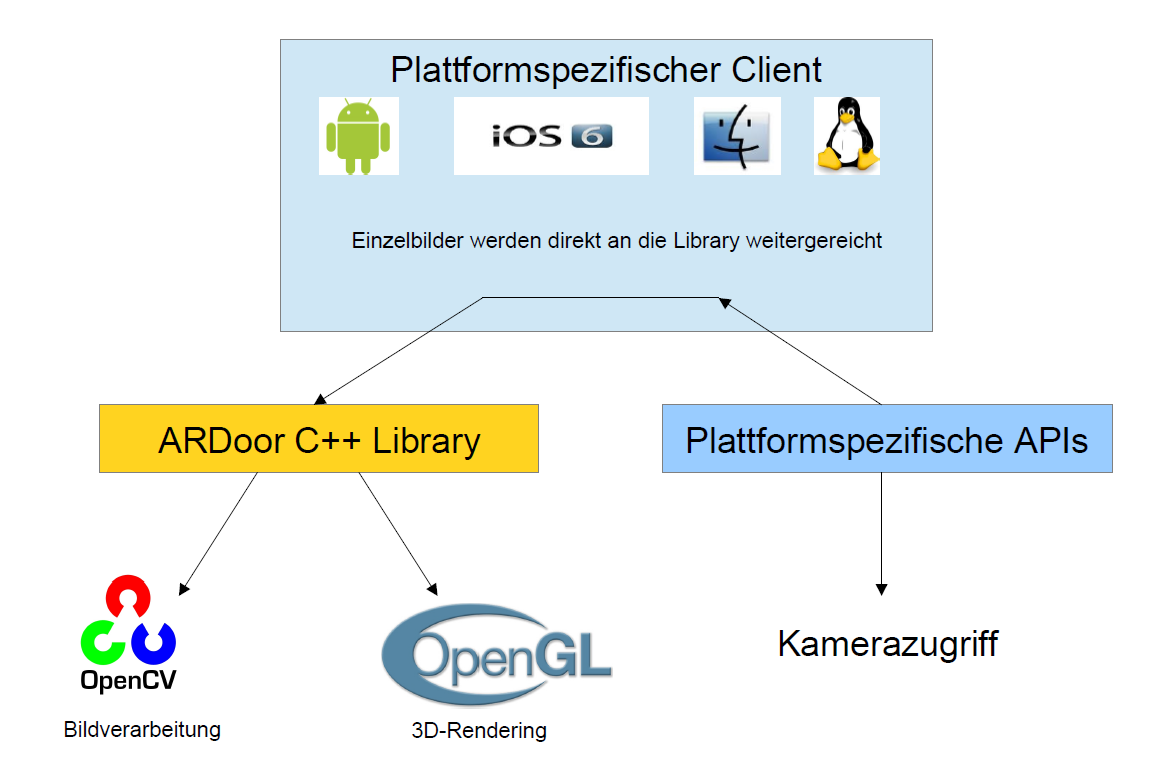
\includegraphics[scale=0.4]{images/architecture.png} 
\caption{Grundarchitektur von ARDoor}
\label{fig:android-architecture}
\end{figure}

\subsection{Android Plattform}
Zur Entwicklung und zum Testen unter Android wurde ein etwas in die Jahre gekommenes HTC Desire Z verwendet. Es wurde jedoch eine Custom Firmware aufgespielt, welche der Android Version 2.3 entspricht, um bessere Native-Unterstützung zu erhalten. Seit dieser Version, welche dem API Level 9 entspricht, gibt es u.a. die Möglichkeit, eine Native Activity zu implementieren.


\subsubsection{Native Activity}
Eine Native Activity ist seit Android 2.3 (API Level 9) verfügbar. Eine Native Activity ist im Grunde ein nützlicher Weg, um eine Android App in C/C++ zu implementieren, ohne noch zusätzlichen Wrapper-Code in Java und JNI Code zu schreiben. Mittels der dem Android NDK beiliegenden Library android\_native\_app\_glue kann das Grundgerüst der Native Activity in C/C++ implementiert werden. Dies hat jedoch einige Probleme bereitet.

\paragraph{}
Eines der Probleme war, dass primär zur Entwicklung unter Android Java (via Dalvik VM) als Programmiersprache vorgesehen ist. Ein Grossteil der verfügbaren APIs ist aus diesem Grund nur über Java aufrufbar. Dazu gehört auch die API für den Kamerazugriff. Es wäre zwar möglich aus C++ über JNI mit der Java-API zu kommunizieren, jedoch ist dies aufwändig und fehleranfällig. Auch verursacht JNI einen gewissen Overhead, wodurch ein Aufruf der rein in Java implementierten APIs aus Java-Code heraus schneller ist. JNI Code ist ausserdem sehr mühsam zum lesen und verursacht hohen Wartungsaufwand.

\paragraph{}
Es gibt auch die Möglichkeit mittels der OpenCV Capture-API auf die Kamera des Smartphone zuzugreifen. Das Problem dabei ist, dass OpenCV dazu nicht dokumentierte Funktionen aus einer Android System-Library aufruft. Dies funktioniert leider nicht mit allen Geräten. Da die aufgerufenen Funktionen nicht zu einer offiziellen, stabilen API gehören, können diese bei einer neuen Android-Version ändern und die Entwickler von OpenCV müssten diese Unterstützung zuerst implementieren.

\paragraph{}
Was bei der Native Activity auch beachtet werden muss ist, dass die ganzen Android-Events, z.B. Input oder App-Lifecycle-Events, selber abgeholt und weiterverarbeitet werden müssen. Dadurch schreibt man quasi von Grund auf ein eigenes Applikationsframework auf nativer Basis.


\subsubsection{JNI Zugriff}
Die andere Möglichkeit ist der Zugriff auf C/C++ via JNI. Die Grund-App wird dabei in Java implementiert. In der nativen Library werden bei dieser Methode spezielle JNI-Funktionen implementiert, die aus Java heraus aufgerufen werden können.

\paragraph{}
Bei dieser Variante haben wir zwar immer noch die Java-Schicht, jedoch kann dadurch auf eine stabile und funktionierende API zurückgegriffen werden. Auch ist es einfacher später ein GUI zu implementieren, z.B. zur Auswahl des zu projizierenden 3D-Models.


\subsection{iOS Plattform}
Zur Entwicklung der iOS Version der Applikation haben wir ein iPhone 4 eingesetzt welches einen A4 Prozessor basierend auf der ARMv7-A\footnote{\url{http://www.arm.com/products/processors/instruction-set-architectures}} Architektur besitzt. Die plattformspezifischen Funktionen wurde in Objective-C geschrieben. Im Gegensatz zu Android braucht es auf der iOS Plattform keine Bridge um C++ Code ausführen zu können. Da Objective-C wie auch C++ eine Obermenge von C ist, können C++ Klassen in der gewohnten Syntax direkt verwendet werden. Dies ist einer der grössten Vorteile der iOS Plattform. Fast alle bestehenden C und C++ Bibliotheken können ohne Umwege Verwendet werden.

\paragraph{}
Einen weiteren Vorteil welchen Objective-C bietet ist, dass alle Klassen grundsätzlich Beliebig erweitert werden können. So konnten wir z.B. die \textit{UIImage} Klasse um Funktionen erweitern, welche es uns ermöglichen den Inhalt eines \textit{UIImage} in eine \textit{cv::Mat} Struktur umzuwandeln und umgekehrt (zu Finden in der Klasse \textit{UIImage+OpenCV}). Somit gestaltete sich der Datenaustausch zwischen den plattformspezifischen Komponenten und unserer unabhängigen ARDoor Library sehr einfach.

\subsubsection{Kamerazugriff} Der Kamerazugriff ist eher etwas komplex gestaltet unter iOS. Glücklicherweise ist die Dokumentation von Apple sehr ausführlich und bietet zu allen komplexen Prozessen Codebeispiele. So auch für den Kamerazugriff. Dies hat uns einiges an Zeit gespart, denn ohne diese Beispiele muss man sehr tiefgehende Kenntnisse – ja man muss schon fast ein Experte sein – von iOS haben um den Kamerazugriff zu konfigurieren. Die Komponenten für Audio und Video In- und Output befinden sich im AVFoundation Framework Welches wiederrum CoreMedia und CoreVideo verwendet (Abb. \ref{fig:avfoundation}).

\begin{figure}[!ht]
\centering
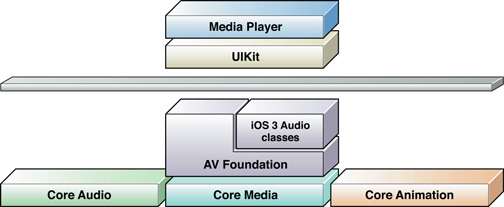
\includegraphics[scale=0.6]{images/avfoundation.jpg} 
\caption{Aufbau des Medienzugriffes unter iOS, Quelle: \url{http://developer.apple.com/library/ios}}
\label{fig:avfoundation}
\end{figure}

Das Setup für den Kamerazugriff gestaltet sich dann wie folgt:

\begin{itemize}
\item Als erstes muss eine Instanz von \textit{AVCaptureDevice} aufgesetzt werden. Diese repräsentiert das Gerät über welches der Input geliefert wird.
\item Über eine \textit{AVCaptureDeviceInput} wird der Datenstrom des Eingabegerätes gesteuert.
\item Mittels \textit{AVCaptureVideoDataOutput} wird die Ausgabe der Daten, in unserem Fall auf ein UIImage, gesteuert.
\item Die letzte Komponente ist die \textit{AVCaptureSession}, welche den Datenstrom von \textit{AVCaptureDeviceInput} zu \textit{AVCaptureVideoDataOutput} steuert.
\end{itemize}

Der Afbau ist in Abb. \ref{fig:ios-capture-overview} visualisiert. Der Code für das Setup befindet sich in \textit{VideoCaptureViewController::createCaptureSessionForCamera}. Obwohl der Kamerazugriff eher komplex aufgebaut ist, bietet er auch einige vorteile. Es ist einfach mehrere Input-Devices wie eine Kamera und ein Mikrofon zusammenzufassen. Weiterhin kann man auch sehr einfach das Input-Device austauschen, z.B. die Backface-Kamera mit der Frontface-Kamera. Beides, ohne dass die darunterliegenden Layer etwas davon mitbekommen.

\begin{figure}[!ht]
\centering
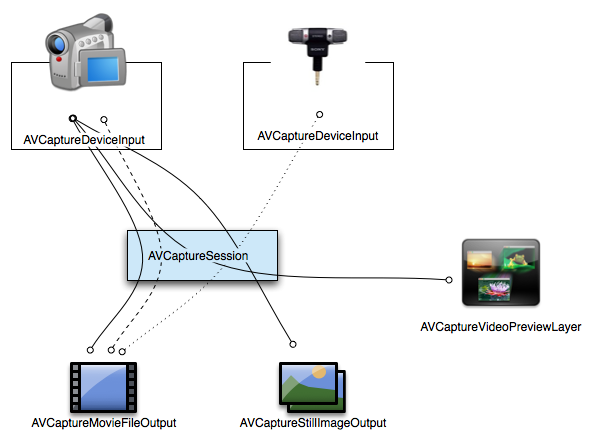
\includegraphics[scale=0.6]{images/ios-capture-overview.png} 
\caption{Aufbau des Medienzugriffes unter iOS, Quelle: \url{http://developer.apple.com/library/ios}}
\label{fig:ios-capture-overview}
\end{figure}

\subsubsection{OpenCV unter iOS}
OpenCV lässt sich unter iOS mittlerweile sehr einfach einbinden. Noch bis vor kurzem musste man die Bibliothek noch selbst für die ARM-Plattform kompilieren, was sich als sehr mühsam erwies. Jedoch bieten die OpenCV-Macher mittlerweile vorkompilerte Binaries in Form eines Framework-Bundles an. Die Framework-Bundle Form hat den Grossen vorteil, dass die Binaries mit relativen Pfaden gelinkt sind. So ist das Deployment viel einfacher. Andernfalls müsste man nach der Kopilierung die Linker-Pfade mittels otool vor dem Deployment anpassen. Eine iOS App wird zuerst lokal auf dem Entwicklungsrechner Kompilert und danach auf das Endgerät (oder den iOS Simulator) installiert. Da die Verzeichnisstrukturen nicht auf beiden Geräten identisch ist, währen somit die Linker-Pfade nicht korrekt wenn sie absolut wären.

\paragraph{Performance} Die Performance von OpenCV unter iOS ist nicht optimal. Innerhalb von OpenCV wird standardmässig OpenMP für die Parallelisierung eingesetzt. Da jedoch OpenMP bisher noch nicht auf ARM portiert wurde, wird die Leistung des Prozessors nicht voll ausgeschöpft. So drückt eine Sobel-Live-Kantendetektion des Kamerabildes die Framerate bereits auf ca. 13 fps runter. Die Erkennung einen Schachbrettmusters mittels \textit{cv::findChessboardCorners} bringt es nicht einmal mehr auf ein fps. Eine Möglichkeit hier die Performance zu Optimieren währe Grand Central Dispatch (GCD) einzusetzen. Dies ist die Objective-C spezifische Multithreading Umgebung von Apple. Seit der Version 2.4.3\footnote{\url{http://code.opencv.org/projects/opencv/wiki/ChangeLog}} besitzt OpenCV eine \textit{parallel\_for} Implementierung für diverse Multithreading Backends, unter anderem auch für GCD. Eine weitere Möglichkeit die Leistung der Anwendung zu optimieren währe, wo möglich, Operationen mittels NEON\footnote{\url{http://www.arm.com/products/processors/technologies/neon.php}} umzusetzen. NEON ist ein SMID Instruction Set, ähnlich wie MMX von Intel, welches parallele Operationen auf einer Instruktion erlaubt. Beide Optionen gilt es während der Bachelor-Thesis zu erforschen.

\subsection{Desktop Platform}
Da die Performance von OpenCV auf den mobilen Geräten suboptimal ist und es auf Grund der tiefen Frameraten sehr mühsam wurde die Applikation zu testen, haben wir uns dazu entschieden auch eine Desktop-Variante umzusetzen. Als Grundlage dafür haben wir das QT-Framework eingesetzt. Zu begin haben wir auch noch eine Mac OS X spezifische App entwickelt. Jedoch wurde der Aufwand zwei Desktop Varianten zu entwickeln schlicht zu hoch, da wir uns in beide Plattformen zuerst tiefer einarbeiten hätten müssen. Deshalb haben wir uns dazu entschlossen, nur noch die QT-Variante weiterzuentwickeln. Mittels QT-Framework kann sowohl unter Mac OS X als auch unter Linux entwickelt werden, welche die Zielplattformen für die Desktop App waren. Einzig bei der Einbindung von Libraries wie OpenCV und bei der Einbindung von einigen Header-Dateien müssen Weichen für OS X und Linux eingebaut werden, da die Namensgebung nicht immer identisch ist. 
\paragraph{}
Eine wichtige Einstellung welche vorgenommen werden musste ist die Deaktivierung des QML-Debuggers. Solange diese Option aktiv war, wurde der eigentliche C++ Debugger nicht korrekt ausgeführt. Das führte dazu, dass Fehler im Code nicht erkannt werden konnten. Die Applikation verhielt sich nicht wie erwartet, gleichzeitig wurden beim Kompilieren aber keine Fehler ausgegeben; Breakpoint wurden einfach ignoriert. Weiterhin verhielt sich das Event-Handling innerhalb von QT nicht wie spezifiziert, solange der QML-Debugger aktiv war. Diese Situation führte zu einer erheblichen Verzögerung in der Entwicklung, bis dieser Konfigurationsparameter als Ursache lokalisiert wurde. Der Grund für dieses Fehlverhalten könnte sein, das wir nicht QML für die Erstellung des UI einsetzen, sondern das XML basierte System. Wahrscheinlich gibt es Inkompatibilitäten zwischen den zwei Libraries.
\paragraph{}
Ein weiteres Hindernis welches wir hatten war die Kompilierung von OpenCV unter Mac OS X. Leider bieten die Hersteller keine precompiled Binaries für Mac OS X an. Das Problem bestand darin, dass der Linker falsche relative Pfade zu OpenCV gesetzt hat. Erst als wir einen Patch für OpenCV\footnote{\url{http://code.opencv.org/issues/2037}} entdeckt hatten, welcher es erlaubte die Bibliothek als Framework zu verpacken, konnte OpenCV problemlos unter Mac OS X betrieben werden. Ein Problem welches bis heute noch ungelöst ist, ist die OpenGL-Unterstützung innerhalb von OpenCV unter Mac OS X. Obwohl der nötige Kompilierungsparameter \textit{WITH\_OPENGL} korrekt gesetzt wurde, wurde OpenCV ohne OpenGL-Unterstützung kompiliert. Dies führte dazu, dass wir viele Beispielapplikationen nicht Ausprobieren, da diese OpenGL-basierte GUIs verwenden.

\subsubsection{Calibration Dialog}
Der Calibration Dialog dient dazu, die Kameraparameter zu ermitteln. Dies muss grundsätzlich nur einmal zu Begin gemacht werden. Die gewonnenen Daten werden anschliessend in eine Konfigurationsdatei abgelegt. Die Datei wird im systemspezifischen Konfigurationsverzeichnis abgelegt.

\subsubsection{Mainwindow}
Das Mainwindow ist der Hauptteil der Applikation. Innerhalb von diesem wird die Augmented Reality Szene dargestellt.

\subsection{ARDoor Library}
Wir haben uns zum Ziel gesetzt, die ARDoor Library möglichst modular aufzubauen, so dass wir verschiedene Komponenten einfach austauschen könnten und wir somit flexibel in der Entwicklung sind. Da wir bei der Entwicklung sehr viele Dinge ausprobiert haben und ständig Sachen neu implementiert haben, konnten wir dies nicht zu 100\% umsetzen. Sobald wir eine erste funktionierende Version mit Positionsbestimmung und korrektem Rendering haben, werden wir ein generelles Code-Refactoring durchführen.

\subsubsection{ImagePipeline}
Eine der Hauptkomponente der ARDoor Library ist die Image Pipeline. Der Grundgedanke dahinter ist, dass die verschiedenen Schritte zur Bildbearbeitung und -verarbeitung in sich geschlossenen modularen Klassen - einem \textit{ImageProcessor} - implementiert werden. Wir erhoffen uns davon eine einfachere Entwicklung, da wir dadurch die verschiedenen Verarbeitungsschritte einfach austauschen oder in der Reihenfolge der Ausführung neu positionieren können.

\paragraph{}
Ein weiterer Grundgedanke für diesen Aufbau war, dass wir so einfach Debugmöglichkeiten einbauen könnten: Man könnte einen einfachen Debug ImageProcessor, der das aktuelle Bild nur darstellt und nicht verändert, implementieren und diesen an eine beliebige Position der Pipline setzen.

\paragraph{}
Implementiert haben wir die Pipeline so, dass für jedes Bild, welches wir von der Kamera erhalten, eine OpenCV-Matrix cv::Mat erzeugt wird. Diese wird der Pipeline nun zur Verarbeitung übergeben. Die Pipeline übergibt diese Matrix dem aktuellen ImageProcessor, der eine weitere Matrix als Rückgabewert liefert. Die zurückgegebene Matrix wird jeweils als Eingabe für den nächsten ImageProcessor in der Pipeline verwendet. Zum Schluss wird von der Pipeline das finale Bild nach allen Verarbeitungsschritten zurückgegeben. Dieser Ablauf ist in Abbildung \ref{fig:image-pipeline} grafisch dargestellt.

\begin{figure}[!ht]
\centering
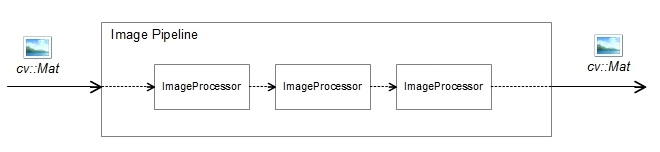
\includegraphics[scale=0.8]{images/image-pipeline.jpg} 
\caption{Aufbau der Image Pipeline}
\label{fig:image-pipeline}
\end{figure}

\subsubsection{RenderingContext}
Eine weitere Komponente der Library ist der RenderingContext. Die primäre Aufgabe dieser Komponente ist das Rendering der 3D-Modelle einer Szene sowie das korrekte setzen der Projektions- und ModelView-Matrizen. Diese strikte Trennung ist im Moment noch nicht konsequent umgesetzt, da der RenderingContext auch Aufgaben der Pose Estimation übernimmt.  

\end{document}
